\chapter{模态自适应医学视觉问答系统实现与在线部署}
在第三章和第四章对阵Med-VQA模型研究的基础上,本章基于人机工程学中的模态自适应原理、结合云服务技术开展系统设计,在云端实现并部署了一个提供医学视觉问答服务的在线模态自适应系统。该系统集成了图像处理、机器翻译等技术组件,
融合传统机器学习、云计算技术、模型部署和服务化技术、自动化运维等技术。使得该系统具备根据当前的上下文环境和用户行为自动适应和调整其模态(Mode)或界面状态的能力;可以根据用户上传或拍摄的图片以及问题,在多个交互模型中进行选择,并给出相应的回答预测。
该云端视觉问答服务稳定、便捷、高效,且支持在线更新。本章内容包括模态自适应系统设计、在线云服务系统设计以及搭建等内容。
%
\section{模态自适应系统}
\subsection{技术路线}
模态自适应系统可以在面临不同输入的复杂场景下,自适应地选择合适的模型与用户完成交互,其主要实现原理是在网络中加入模型控制单元,通过输出反馈和学习算法对输入和系统状态关系进行建模并训练相应的控制模型,让控制模型自主学习合适的交互策略。
同时也能在这一闭环内建立完整的对话样本采集学习的内环回路,在实现模型自适应交互的基础上还可以完成对话样本的高效收集。
\begin{figure}[htbp]
	% 图片居中(列居中对齐)
	\centering	
	% 包含当前路径下的Fig文件夹的图片文件
	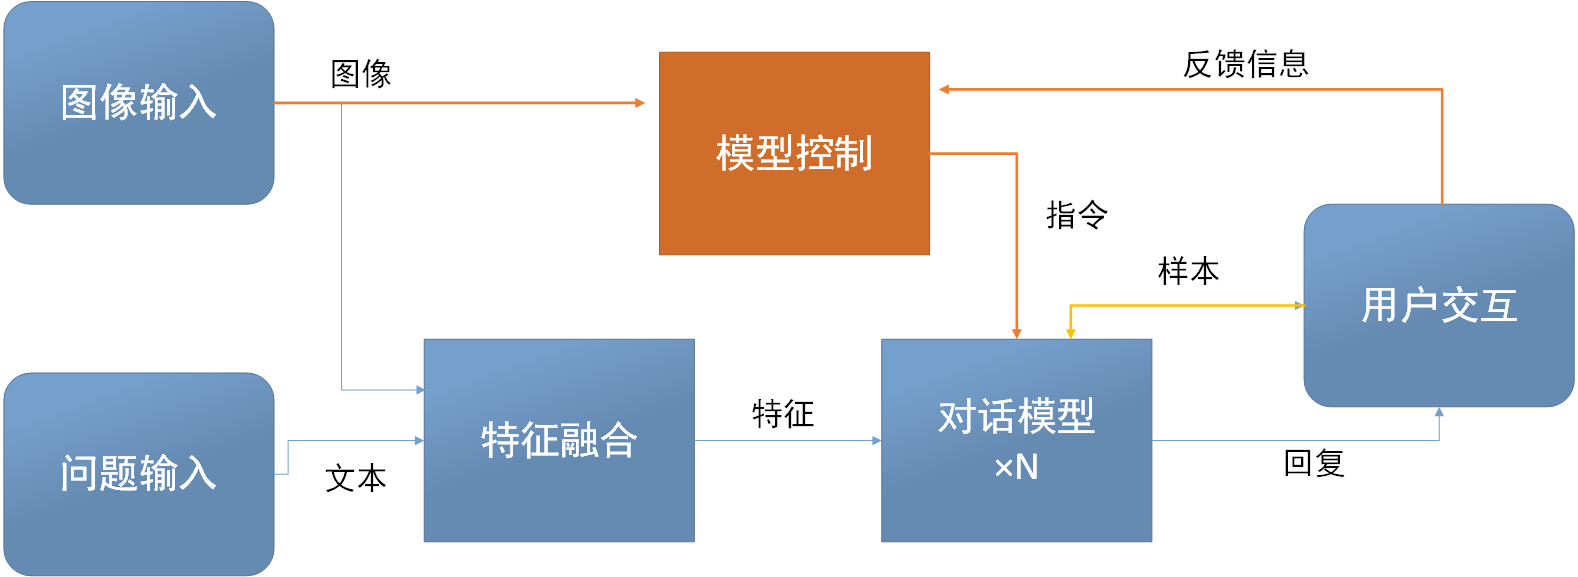
\includegraphics[width=0.8\textwidth]{Fig/myfig/chapter5/sys_febroot.png}  %scale = 0.3
	% 添加标签one_DFUAV以及图标题“XXX”,引用某图时使用\ref{xxx},其中xxx就是标签,图编号是自动生成的。
	\caption{\label{sys_need}模态自适应Med-VQA系统实现技术路线} 
\end{figure}
如图\ref{sys_need},在传统的对话路线之外,新增加了对图像输入-对话模型之间的关联控制,通过一些轻量化的机器学习算法或经典的分类网络在不同类型的图像输入和相应的对话模型之间建立关联,通过用户对话反馈以及输出的不确定性设计
反馈逻辑获得可用于训练的对话决策样本,从而获得在面临不同医学图像输入(例如放射学、病理学)模型可以自主识别用户的输入类型并选择合适的对话策略。这个设计思想和“专人专攻”的思想相近似,其优势是不用重新设计和训练可以处理多种不同数据特征的多模态“大模型”,
这种方式不仅代价高昂并且由于样本之间的互相干扰,模型很难学习到合适的特征对其进行划分,往往也会导致各类型任务的分类性能下降。另一方面,也避免了必须独立使用具有相似功能的模型的情况,提高了系统功能的集成化。
所以模态自适应技术可以在一个独立系统内将用于处理各个模态的轻量化模型进行高效集成,从而在保证各个子系统原本性能的同时,解放了输入数据的限制,提高了模型的泛化能力和交互体验。

\subsection{设计原理}
在多模型交互的场景下,可以基于规则、检索等传统方式选择合适的交互模型,但这种模型是固定的逻辑,存在泛化能力弱不具备自主调节能力等弊端。如图\ref{comu_logit}基于机器学习方法搭建的模型控制器可以根据用户或者系统的反馈,实现一个可自适应的对话模型控制器,可根据用户的输入和反馈将问题分类到
合适的模型中进行处理。而多模型的集成(例如投票、加权)也可以提高系统的准确性和鲁棒性,以及根据用户的反馈,不断对模型进行调整和优化,以提高对话系统的性能和用户体验。

\begin{figure}[htbp]
	% 图片居中(列居中对齐)
	\centering	
	% 包含当前路径下的Fig文件夹的图片文件
	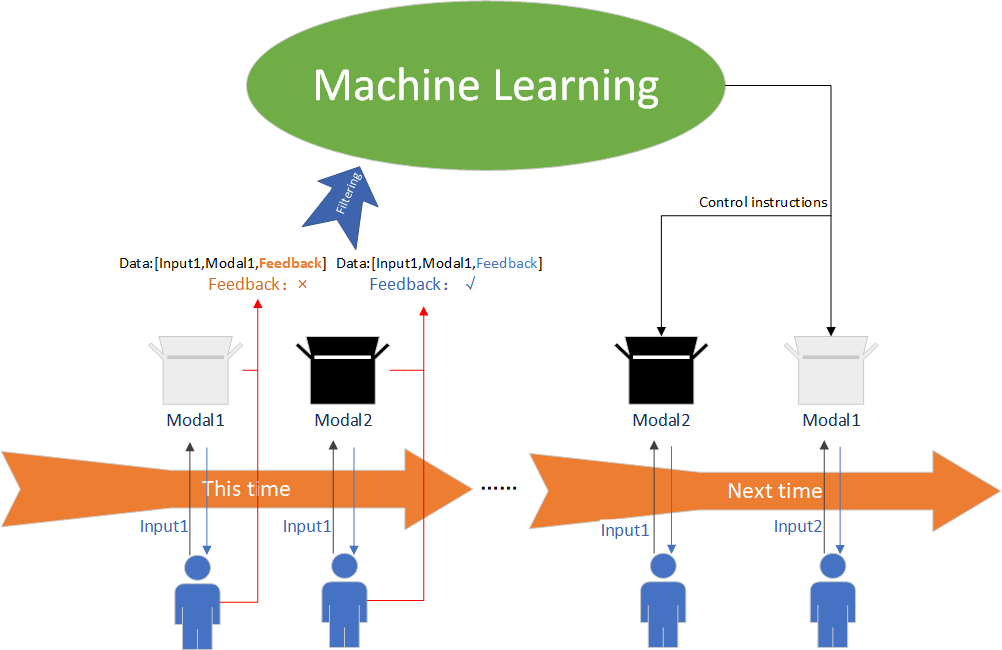
\includegraphics[width=0.8\textwidth]{Fig/myfig/chapter5/comu_logit.png}  %scale = 0.3
	% 添加标签one_DFUAV以及图标题“XXX”,引用某图时使用\ref{xxx},其中xxx就是标签,图编号是自动生成的。
	\caption{\label{comu_logit}自适应交互逻辑} 
\end{figure}

在现有的公开医学视觉问答数据集中,主要是放射学和病理学两个类别的数据,针对每个类型的数据和数据集都可以采用第三、四章节的方法训练出一个性能较为优秀并且带不确定性预测的MedVQA模型,如MEMSA-RAD模型、MEMSA-SLAKE模态等。自适应系统通过多模型选择、用户反馈、模型策略优化、模型集成和迭代等步骤逐渐获得最优的效果,即时是
面对复杂抽象的输入,只要获得正确的反馈并加以迭代,模型也能够对其进行识别和适应。

如图\ref{sys_model},依据系统预设的自适应交互逻辑,在检索式模型回答具有低不确定性的情况下,模型会优先使用检索式模型以获得更为准确,专业的医学回答。
在面对高不确定的回答场景,检索式模型会切换成关闭状态,向模型控制器反馈拒绝分类信号并将原始输入传递给生成式模型。模型控制器在接收到拒绝分类信号后会启用生成式模型,以获得更丰富,具有更好交互效果的生成式回答。
\begin{figure}[htbp]
	% 图片居中(列居中对齐)
	\centering	
	% 包含当前路径下的Fig文件夹的图片文件
	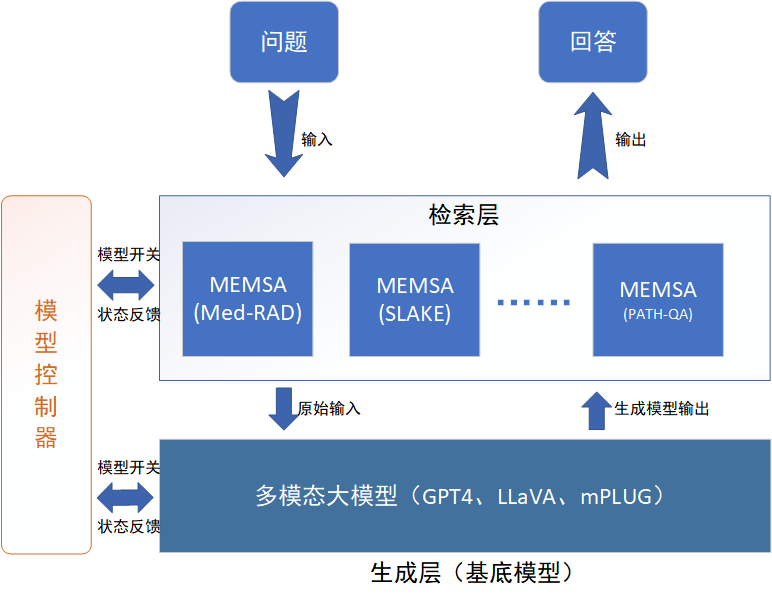
\includegraphics[width=0.8\textwidth]{Fig/myfig/chapter5/sys_model.png}  %scale = 0.3
	% 添加标签one_DFUAV以及图标题“XXX”,引用某图时使用\ref{xxx},其中xxx就是标签,图编号是自动生成的。
	\caption{\label{sys_model}模态自适应系统设计} 
\end{figure}

这种设计方案充分结合了检索模型响应快,效率高,回答针对性强,准确性好以及生成模型回答内容丰富,交互效果好的优点。
同时也巧妙规避了互相之间的缺点,比如在用户进行任务式对话的场景下,选用检索式模型可以规避掉生成模型响应慢,回复冗余等缺点。
在闲聊式场景下,选用生成式模型可以避免检索式模型答非所问的尴尬情况,同时生成式模型强大的上下文能力也有助于对话更好地开展。

\subsection{系统表现}
经上述原理设计的Med-VQA系统,其表现如图\ref{sys_adaptive},当用户提问是否有肿瘤这种任务性明显的对话时,系统进入检索模式,并给出
具有较低不确定性的回答,当用户发起“图中是什么情形?”这种可具备多重解释的开放式闲聊对话时,系统会进入生成模式,给出较为完整的回答。
\begin{figure}[htbp]
	% 图片居中(列居中对齐)
	\centering	
	% 包含当前路径下的Fig文件夹的图片文件
	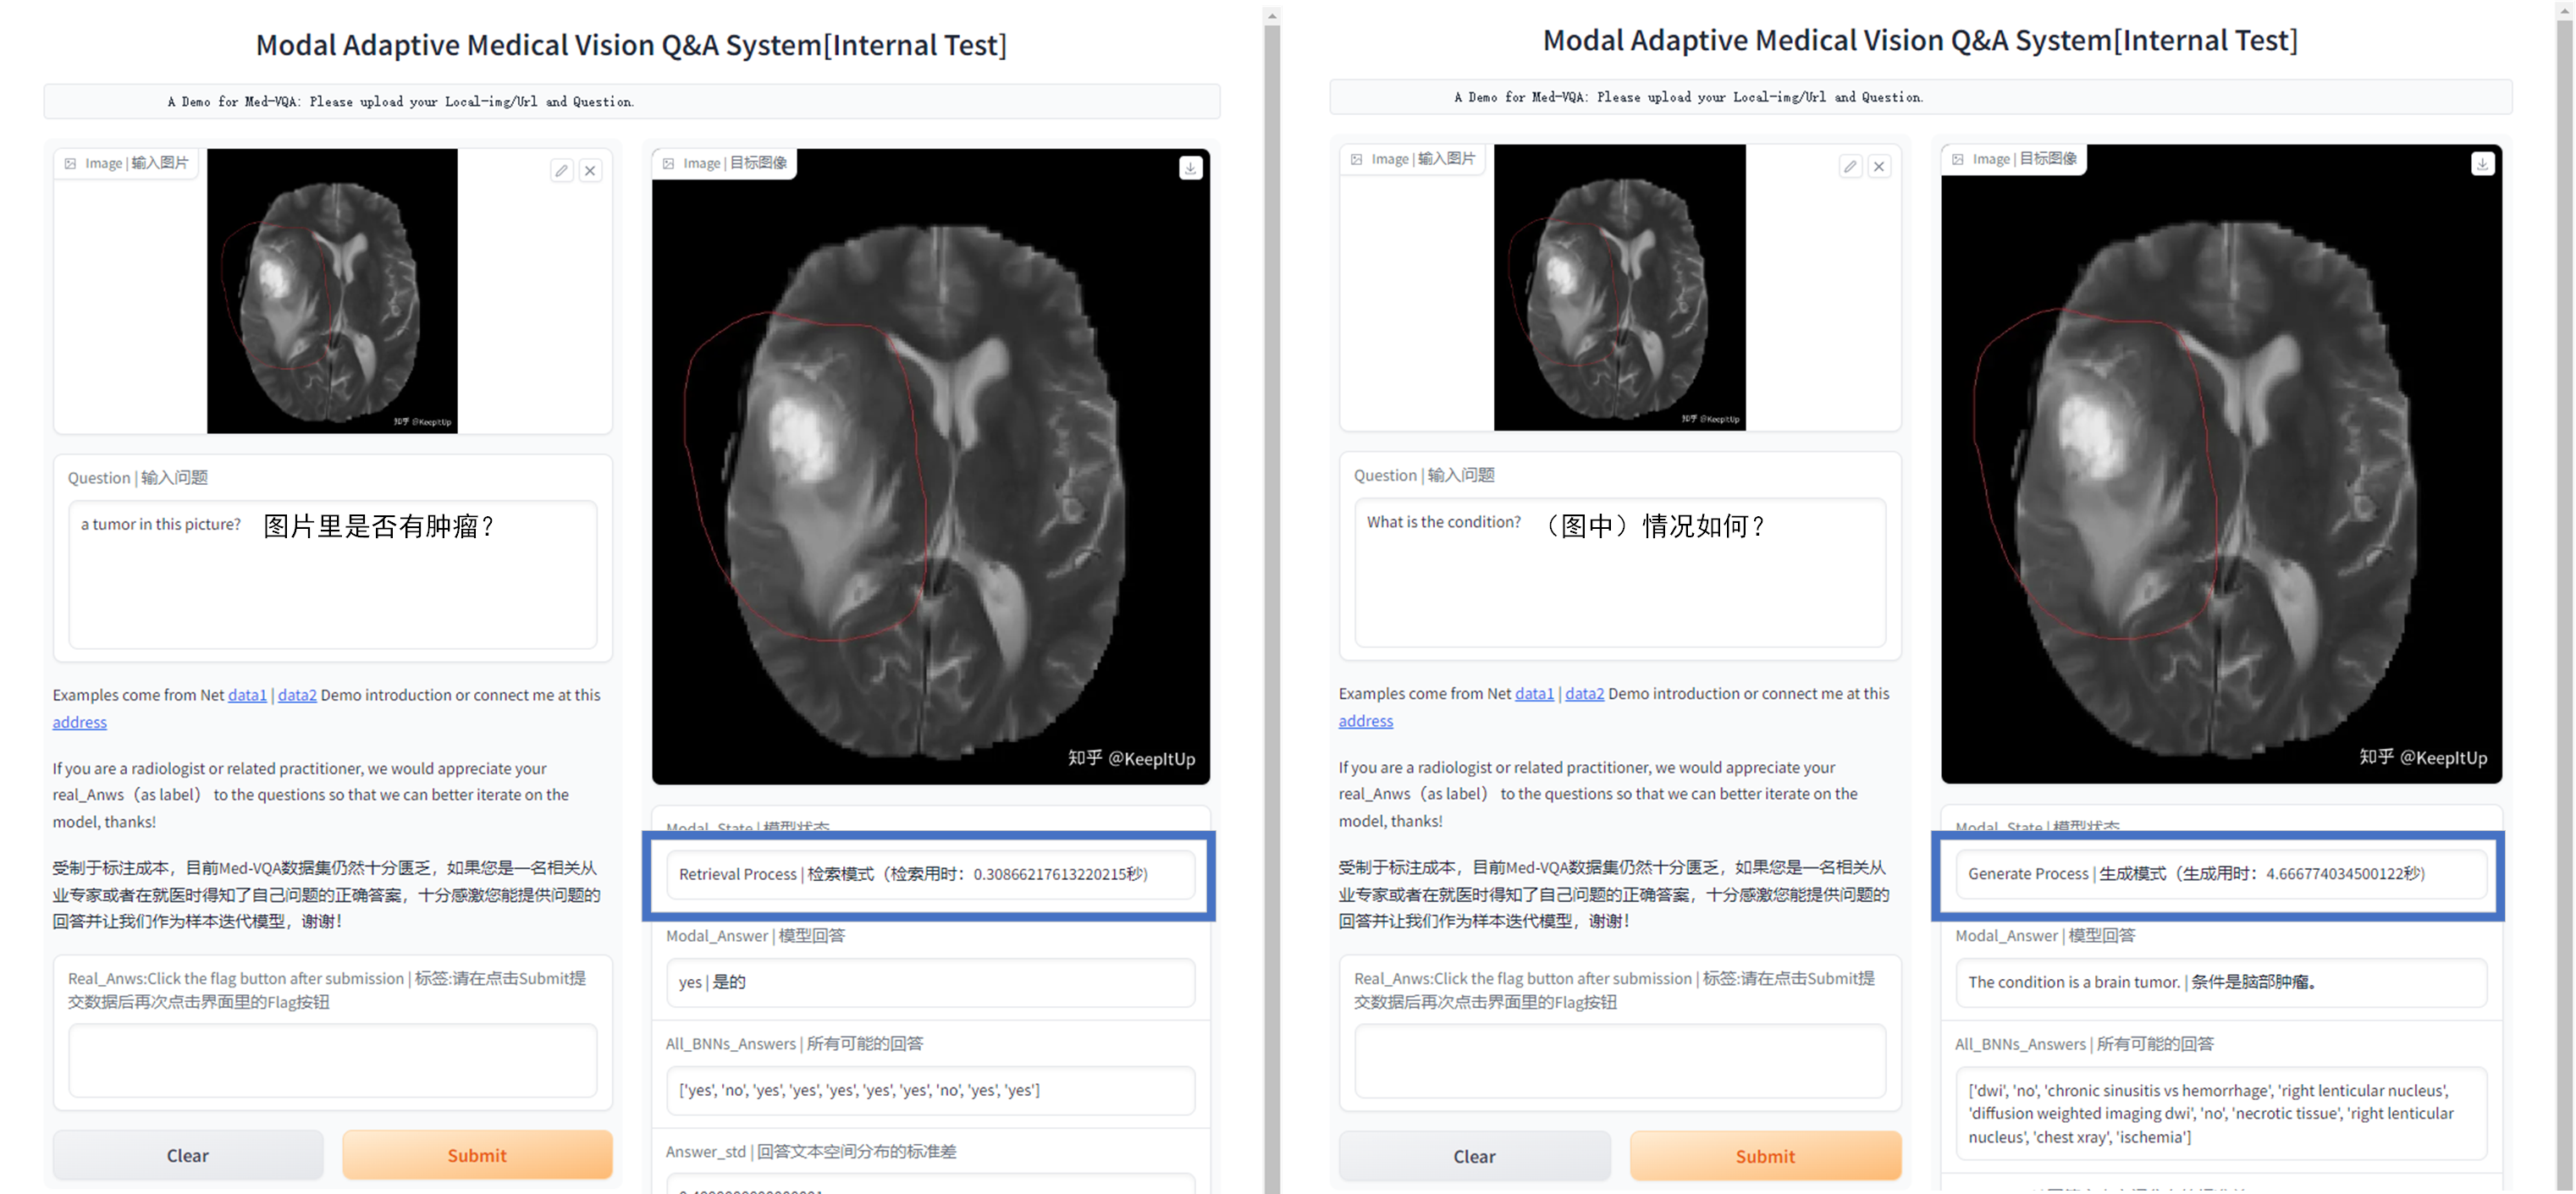
\includegraphics[width=1\textwidth]{Fig/myfig/chapter5/sys_adaptive.png}  %scale = 0.3
	% 添加标签one_DFUAV以及图标题“XXX”,引用某图时使用\ref{xxx},其中xxx就是标签,图编号是自动生成的。
	\caption{\label{sys_adaptive}Med-VQA自适应问题输入使用不同的回答模型} 
\end{figure}

为了更直观地体现出检索式模型和生成式模型在Med-VQA问答时的差异和优劣,如图\ref{fig_compare}从Med-VQA测试集中随机抽取了5个测试样例P1~P5,并用其问题同时测试所提出的检索式模型MEMSA
和目前前沿的生成式模型MiniGPT4\cite{zhu2023minigpt},从测试结果如表\ref{tab:LLMmodal_compare}中可以得到,现有的图文多模态大模型仍然只能够传统VQA中的看图说话,回答语言-自然图像的关联性任务,
但无法准确回答专业性较高的医学诊断问题。
\begin{figure}[htbp]
	% 图片居中(列居中对齐)
	\centering	
	% 包含当前路径下的Fig文件夹的图片文件
	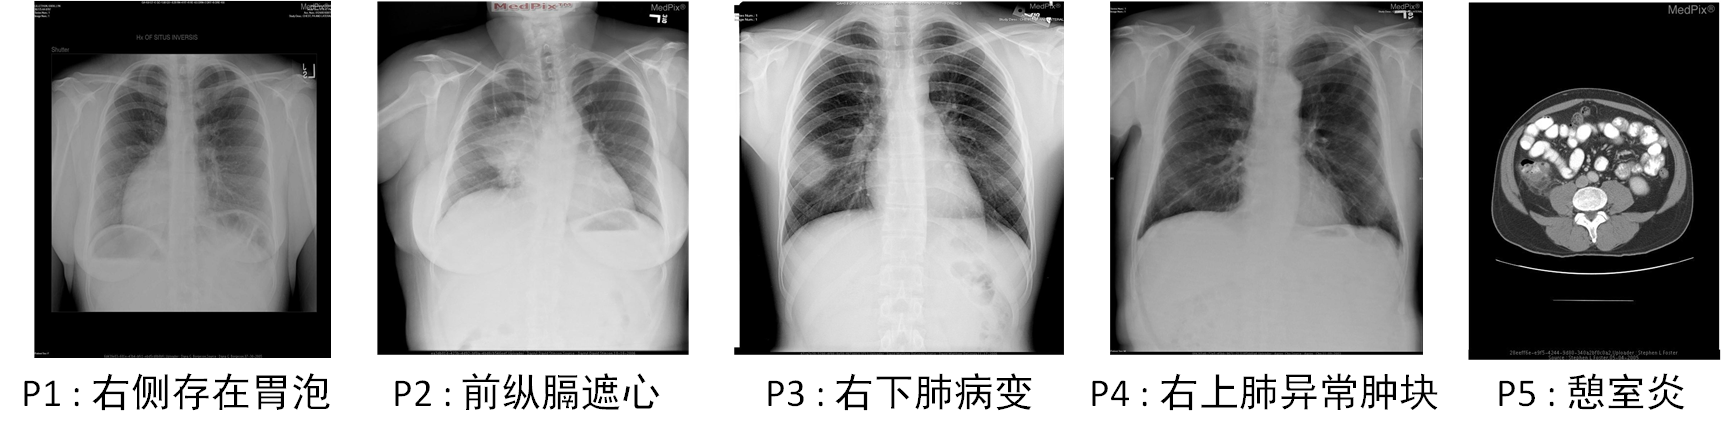
\includegraphics[width=1\textwidth]{Fig/myfig/chapter5/fig_compare.png}  %scale = 0.3
	% 添加标签one_DFUAV以及图标题“XXX”,引用某图时使用\ref{xxx},其中xxx就是标签,图编号是自动生成的。
	\caption{\label{fig_compare}检索式模型和生成式大模型Med-VQA对比图像样例} 
\end{figure}

\begin{table}
	\caption{\label{tab:LLMmodal_compare}检索式模型和生成式大模型Med-VQA对比(√:有效回答|×:无效回答)}
	\centering
	\small
	% \begin{tabular}{|c|c|c|c|c|}
	% 	\hline image & question & answer-lable & predicted-answer-MEMSA & predicted-answer-MiniGPT4 \\
	% 	\hline \multirow{5}{*}{ P1 } & Is there a rib fracture? & No & no & The rib fracture is located on the right side of the chest. \\
	% 	& Is there evidence of any fractures of the ribs? & No & no & There is $no evidence$ of any fractures of the ribs. \\
	% 	& Is there any intraparenchymal abnormalities in the lung fields? & No & no & There is $no evidence$ of any intraparenchymal abnormalities in the lung fields. \\
	% 	& Is there evidence of any abnormalities of the lung parenchyma? & No & no & There is $no evidence$ of any abnormalities of the lung parenchyma. \\
	% 	& Is the gastric bubble shown on the left or right side of the patient? & Right side & right side & The gastric bubble is shown on the right side of the patient. \\
	% 	\hline \multirow{2}{*}{ P2 } & Where is the lesion located? & Anterior mediastinum & anterior mediastinum & The lesion is located on the right lung. \\
	% 	& Which side of the heart border is obscured? & Right & right & The left side of the heart border is obscured. \\
	% 	\hline \multirow{3}{*}{ P3 } & Is there air present under the diaphragm? & No & no & $Yes, there is air present under the diaphragm.$ \\
	% 	& What is the location of the lesion? & right lower lateral lung field & right lower lateral lung field & The location of the lesion is in the chest. \\
	% 	& Where is the lesion located? & right lower lateral lung field & right lower lateral lung field & The lesion is located in the chest. \\
	% 	\hline \multirow{7}{*}{ P4 } & How large is the mass in the right upper quadrant? & 3. $4 \mathrm{~cm}$ & The mass in the right upper quadrant is $not visible$ in the image. The image only shows the inside of the lungs and heart. \\
	% 	& Size of the mass in the right upper quadrant? & $3.4 \mathrm{~cm}$ & no & The mass in the right upper quadrant is $not visible$ in the image. The image only shows the inside of the lungs and heart. \\
	% 	& Is the heart enlarged? & No & no & It is $not possible to determine$ from this image if the heart is abnormally large or not. The image only shows the inside of the lungs and heart, and does not provide any information about the size of the heart. \\
	% 	& Is the heart abnorma11y large? & No & no & It is $not possible to determine$ from this image if the heart is abnormally large or not. The image only shows the inside of the lungs and heart, and does not provide any information about the size of the heart. \\
	% 	& In which lobe do you see an abnormal mass in the above images? & Right upper lobe & right upper lobe & It is $not possible to determine$ from this image if there is an abnormal mass in either lobe of the lungs. The image only shows the inside of the lungs and heart, and does not provide any information about the presence of a mass \\
	% 	& Where is the abnorma1 mass located with respect to the lungs? & Right upper lobe & right upper lobe & It is $not possible to determine$ from this image where an abnormal mass is located with respect to the lungs. The image only shows the inside of the lungs and heart, and does not provide any information about the location of a mass. \\
	% 	& What imaging modality was used to take this image? & Xray & xray & It is $not specified$ what imaging modality was used to take the image. The image itself does not provide any information about the type of imaging modality used. \\
	% 	\hline \multirow{3}{*}{ P5 } & What is the condition? & Diverticulitis & diverticulitis & The condition is $not specified$ in the image. The image is a generic CT scan of the abdomen and does not show any specific details or conditions. \\
	% 	& What is the pathology? & Diverticulitis & diverticulitis & The pathology is $not specified$ in the image. The image is a generic CT scan of the abdomen and does not show any specific details or conditions. \\
	% 	& Can the patient's encephalon be seen in this image? & & yes & $No, the patient’s encephalon cannot be seen in this image.$ The image is a generic CT scan of the abdomen and does not show any specific details or conditions related to the brain or encephalon. \\
	% 	\hline
	% 	\end{tabular}
	\begin{tabular}{|c|c|c|}
		\hline Img & question & lable/ans(MEMSA|MiniGPT4)\\
		\hline \multirow{5}{*}{ P1 } & Is there a rib fracture? & No/(√ | ×) \\
		& evidence of any fractures of the ribs? & No/(√ | √)\\
		& any intraparenchymal abnormalities in the lung fields? & No/(√ | √) \\
		& evidence of any abnormalities of the lung parenchyma? & No/(√ | √) \\
		& gastric bubble shown on the left or right side of the patient? & Right side/(√ | √) \\
		\hline \multirow{2}{*}{ P2 } & Where is the lesion located? & Anterior mediastinum/(√ | ×) \\
		& Which side of the heart border is obscured? & Right/(√ | √) \\
		\hline \multirow{3}{*}{ P3 } & Is there air present under the diaphragm? & No/(√ | ×) \\
		& What is the location of the lesion? & right lower lateral lung field/(√ | ×) \\
		& Where is the lesion located? & right lower lateral lung field/(√ | ×) \\
		\hline \multirow{7}{*}{ P4 } & How large is the mass in the right upper quadrant? & $3.4 \mathrm{~cm}$/(√ | ×) \\
		& Size of the mass in the right upper quadrant? & $3.4 \mathrm{~cm}$/(× | ×) \\
		& Is the heart enlarged? & No (√ | ×) \\
		& Is the heart abnorma11y large? & No/(√ | ×) \\
		& In which lobe do you see an abnormal mass? & Right upper lobe/(√ | ×) \\
		& Where is the abnorma1 mass located with respect(lungs)? & Right upper lobe/(√ | ×) \\
		& What imaging modality was used to take this image? & Xray/(√ | ×) \\
		\hline \multirow{3}{*}{ P5 } & What is the condition? & Diverticulitis/(√ | ×) \\
		& What is the pathology? & Diverticulitis/(√ | ×) \\
		& Can the patient's encephalon be seen in this image? & No/(× | ×) \\
		\hline
		\end{tabular}
\end{table}

相比于GPT等生成式大模型,采用检索式方案的Med-VQA模型可以用较少的参数对医学问答样本进行训练获得。对于Med-VQA这种任务式占主要的问答场景,检索式模型的分类特性也能够提供相对更准确高效的回复从而完成用户的提问任务。答案相对固定,且要求模型准确、高效,这是Med-VQA不同与VQA的主要区别,
与也是目前主流Med-VQA依然采用检索式方案的原因。

\section{讨论}
\subsection{模型控制学习算法}
基于现有的医学问答场景问答诉求,主要的图像输入如\ref{dataexm}为放射学图像以及病理学图像。为了让系统学会自主区分这两种模态的图像输入,综合对比了目前常见的机器学习图像分类算法以及系统响应性能。
在测试中表现出准确率高,系统响应快,具有实时调整能力的机器学习算法模型通常是使用在即时对话系统中进行模型控制的较好选择。为了训练并初始化这个图像分类器,选用了Med-RAD中的所有放射学图像315张以及
Path数据集中的前315张病理学图像,总计630张组成一个新的数据集并按8:2的比例划分训练集和测试集,其所在的数据集作为每张图片的分类标签,选用不同的分类模型进行分类。
\begin{figure}[htbp]
	% 图片居中(列居中对齐)
	\centering	
	% 包含当前路径下的Fig文件夹的图片文件
	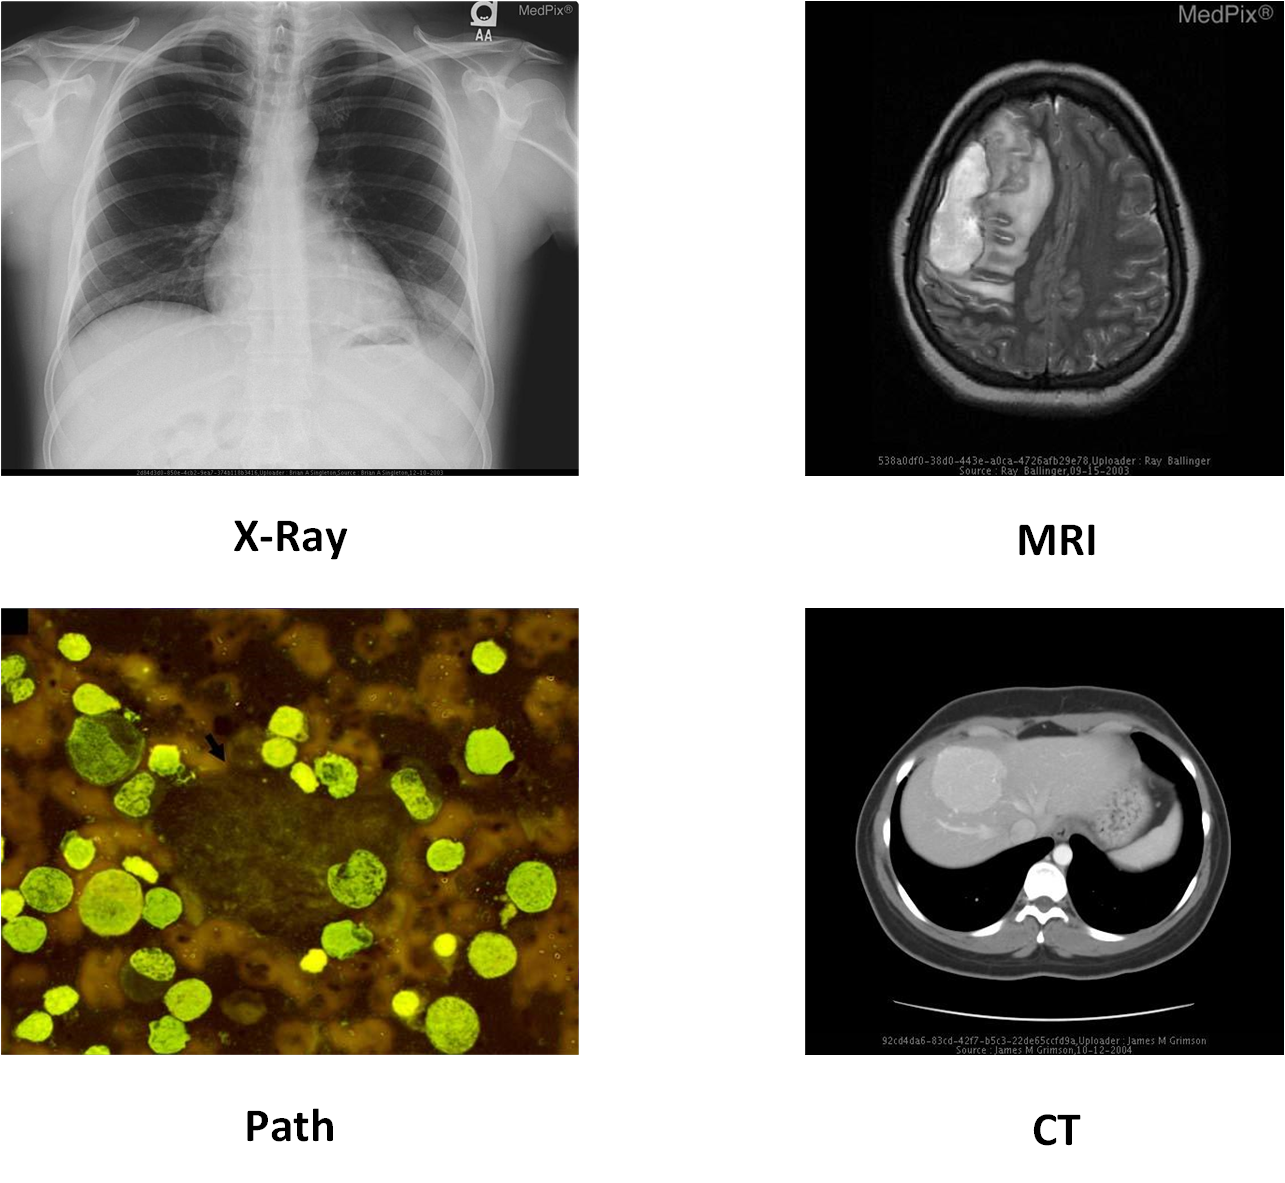
\includegraphics[width=0.8\textwidth]{Fig/myfig/chapter5/dataexm.png}  %scale = 0.3
	% 添加标签one_DFUAV以及图标题“XXX”,引用某图时使用\ref{xxx},其中xxx就是标签,图编号是自动生成的。
	\caption{\label{dataexm}输入各模态数据样例} 
\end{figure}

最终在测试集上的性能表现如表\ref{tab:ML_compare}。
\begin{table}
	\caption{\label{tab:ML_compare}不同机器学习算法的性能评估对比}
	\centering
	\small
	\begin{tabular}{c|cccccccc}
		\hline  方法 & TN & FP & FN & TP & Acc & Precision & Recall & F1 \\
		\hline 朴素贝叶斯 & 48 & 7 & 10 & 61 & 0.865 & 0.897 & 0.859 & 0.876 \\
        决策树(avg) & 54 & 1 & 4 & 69 & 0.960 & 0.985 & 0.943 & 0.964 \\
        感知机 & 51 & 4 & 0 & 71 & 0.968 & 0.947 & 1.0 & 0.973 \\
        逻辑回归 & 51 & 4 & 0 & 71 & 0.968 & 0.946 & 1.0 & 0.972 \\
		支持向量机 & 52 & 3 & 0 & 71 & 0.976 & 0.959 & 1.0 & 0.979 \\
        随机森林 & 55 & 0 & 2 & 69 & 0.984 & 1.0 & 0.972 & 0.986 \\
		\hline
		\end{tabular}
\end{table}
经过对比,当随机森林算法作为模型控制器,也就是用于选择不同Med-VQA模型的控制算法时具有最好的准确率、精确率和F1值,且在此类无正负例倾向的分类场景中,准确率和F1分数为最主要的参考指标,且随机森林算法在防止过拟合、鲁棒性和可解释性上相比其他算法也有一定的优势,
故而选择随机森林算法作为模型自适应控制的学习算法。

\subsection{实验分析}
综上所述,该模态自适应系统设计可以自适应地在不同医学影像输入间进行转换和交互。它可以使得机器学习模型能够在多种输入模态下进行训练和推断,从而提高了模型的鲁棒性和实用性。但同时,
这个系统本身也存在一定的不足之处。例如,接受反馈以及模型调整存在明显的滞后效应,单个用户往往不会询问一个问题多次。其次就是反馈的数据并不能直接用于训练,还需要专业的医生进行筛选甄别,
这无形中会增大其成本。并且要想达到很好的跨模态效果,还需要大量相关数据的支持,这也是现医学视觉问答领域面临的主要挑战。

\section{在线云服务VQA系统}
\subsection{系统功能性需求}
协助用户完成视觉问答任务是一个VQA系统的核心功能。通常来说,这个系统由系统管理、信息处理和问答模型三个部分构成。系统管理主要负责系统日志控制,系统内外部的信息通信;信息处理负责对系统输入
的图像或者文本信息以及数据流进行预处理,转换成问答模型所需要的信息格式;VQA模型是本系统的核心模块,包括模型控制、模型问答两部分。所设计的系统总体功能需求如图\ref{sys_need}。
\begin{figure}[htbp]
	% 图片居中(列居中对齐)
	\centering	
	% 包含当前路径下的Fig文件夹的图片文件
	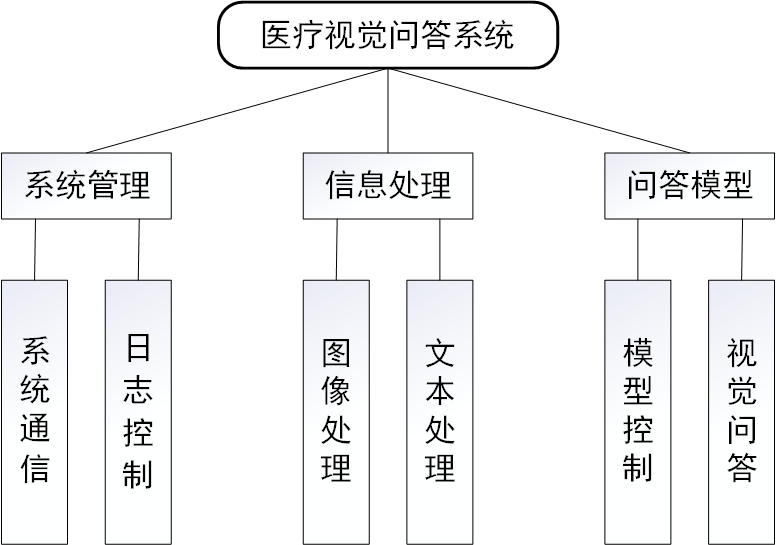
\includegraphics[width=0.6\textwidth]{Fig/myfig/chapter5/sys_need.png}  %scale = 0.3
	% 添加标签one_DFUAV以及图标题“XXX”,引用某图时使用\ref{xxx},其中xxx就是标签,图编号是自动生成的。
	\caption{\label{sys_need}需求分析} 
\end{figure}
由于该系统的主要交互角色是用户和VQA模型,下面通过图例具体介绍这两种角色涉及到的功能模块:
\begin{enumerate}[topsep = 0 pt, itemsep= 0 pt, parsep=0pt, partopsep=0pt, leftmargin=0pt, itemindent=44pt, labelsep=6pt,  listparindent=22pt, label=(\arabic*)]
    \item 用户用例如图\ref{eg_user},对于使用本系统的用户,系统主要负责处理用户的信息采集以及完成问答请求。其中信息采集包括用户上传的医学影像图片以及相对应的问题,其中这两个输入都要做到良好的兼容性,
    图像采集需做到兼容常见的图像格式和资源形式,例如兼容png、jpg等格式的图片以及用户采用的是本地上传或者是网络资源定位符url的方式提供图像信息。问题文本采集
	应充分考虑语种,语言类型的差异,对不同语种问题的输入,接口需具备基础的翻译能力。同时在处理问答请求是要区分是控制请求还是服务请求,控制请求分为API调用或者前端调用
	两种不同的服务请求,确认后系统才能够提供准确的返回形式。服务请求则需要系统调用视觉问答模型对问题输入进行回复,为用户提供服务。
    \begin{figure}[htbp]
        % 图片居中(列居中对齐)
        \centering	
        % 包含当前路径下的Fig文件夹的图片文件
        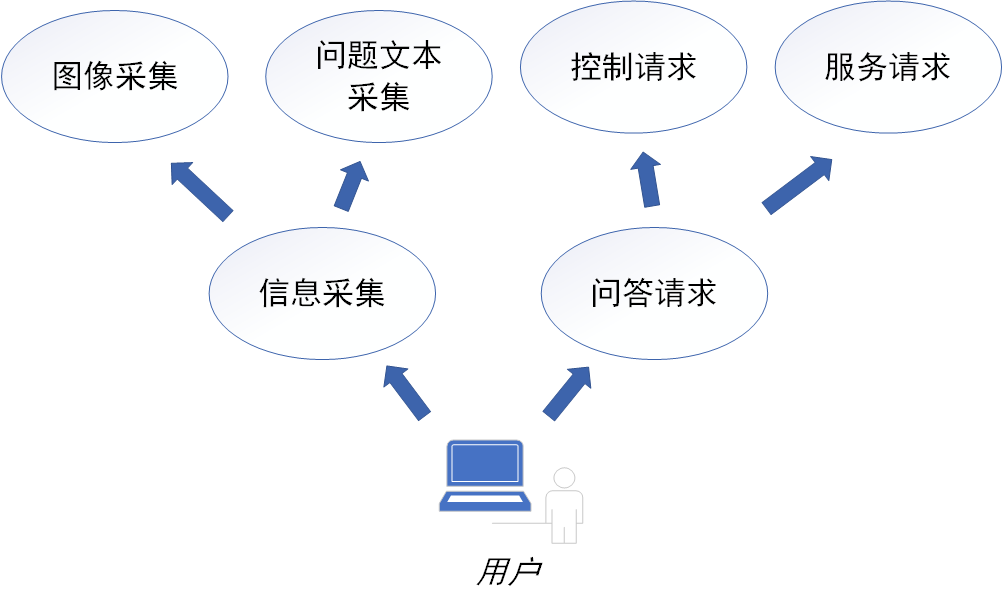
\includegraphics[width=0.8\textwidth]{Fig/myfig/chapter5/eg_user.png}  %scale = 0.3
        % 添加标签one_DFUAV以及图标题“XXX”,引用某图时使用\ref{xxx},其中xxx就是标签,图编号是自动生成的。
        \caption{\label{eg_user}用户用例} 
    \end{figure}
    \item 模型用例如图\ref{eg_model},对于搭载在系统上视觉问答模型,系统主要通过各种接口为其实现机器翻译,答案返回(云端下发)以及样本收集等功能。在面对非英语输入时,系统需要调用翻译组件进行翻译,最后交由模型进行问答,
    当模型返回答案预测时,系统会将其整理成带标签的字典,并打包成JSON信息下发给用户。在面对需要收集的样本时,系统先将数据按样本和标签进行分类整理,并调用本地OS将其保存在数据文件夹或者数据库文件中。
    \begin{figure}[htbp]
        % 图片居中(列居中对齐)
        \centering	
        % 包含当前路径下的Fig文件夹的图片文件
        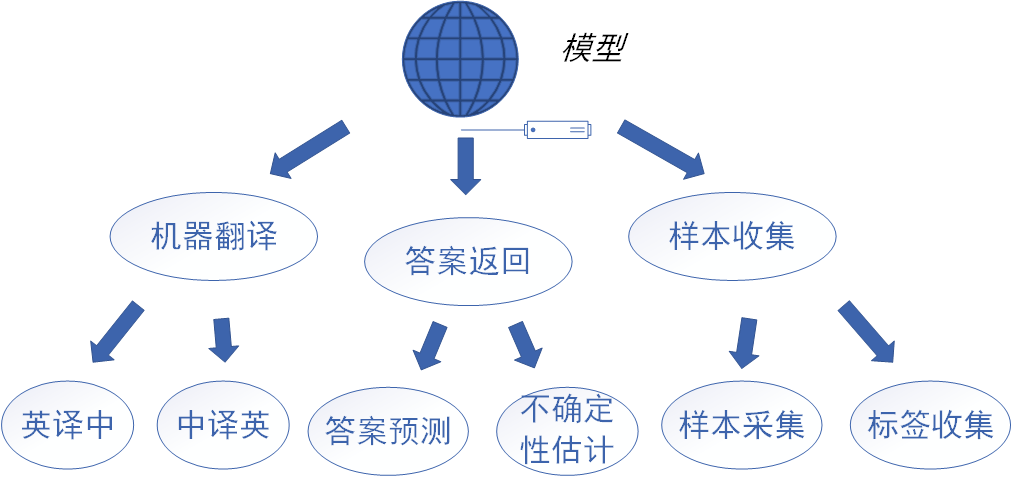
\includegraphics[width=0.8\textwidth]{Fig/myfig/chapter5/eg_model.png}  %scale = 0.3
        % 添加标签one_DFUAV以及图标题“XXX”,引用某图时使用\ref{xxx},其中xxx就是标签,图编号是自动生成的。
        \caption{\label{eg_model}VQA模型用例} 
    \end{figure}
\end{enumerate}

\subsection{非功能性需求}
除了完成核心功能,系统还需要满足其他功能要求以确保运行的实用性和可靠性,这些要求称为非功能性需求。视觉问答系统的非功能性需求主要包括高可用性和高响应性。
如果是处于生产环境部署的情况下,同时要考虑到其安全性和可扩展性。

高可用性又包涵高可靠性、灵活性以及可视化等几个特点。高可靠性是指模型需要在面对各种异常情况(如网络延迟、服务器故障等)时保证系统的稳定性;灵活性是指模型
具备灵活部署、维护和升级的能力,以适应不同业务场景的需求;可视化则要求模型具备可视化的特点,能够为用户提供直观,清晰的结果展示,以便用户更好的使用和理解模型。
由于视觉问答系统内部模型复杂,集成算法较多,出现故障的可能性极高。为此采用分布式多机部署的方案来保证系统的可靠性和高可用性。

高响应性是指系统具有快速响应用户操作和请求的能力,包括用户界面的快速响应、数据的快速检索和处理等。对于需要实时性比较高的模型,需要在部署时考虑响应性问题,
以确保良好的用户反馈和用户体验。为了缩短视觉问答模型中的特征提取和答案推理过程所需的响应时间,可以考虑采用缓存数据的方式来减少数据读取和存储的时间。
同时,使用消息队列技术可以实现削峰、解耦以及异步处理系统的其他功能(例如日志存储),从而防止信道阻塞并避免增加核心功能VQA的响应时间。
\subsection{总体架构}
总体设计分为服务端和客户端两大模块,服务端组织构成上包含后端服务器和代理服务器,开放API访问接口以及相关技术文档提供服务,由服务端主机在内网发布,再
通过内网穿透+代理服务器开放到公网提供外部访问,客户端则是一些前端交互实现,总体架构如图所示。
\begin{figure}[htbp]
	% 图片居中(列居中对齐)
	\centering	
	% 包含当前路径下的Fig文件夹的图片文件
	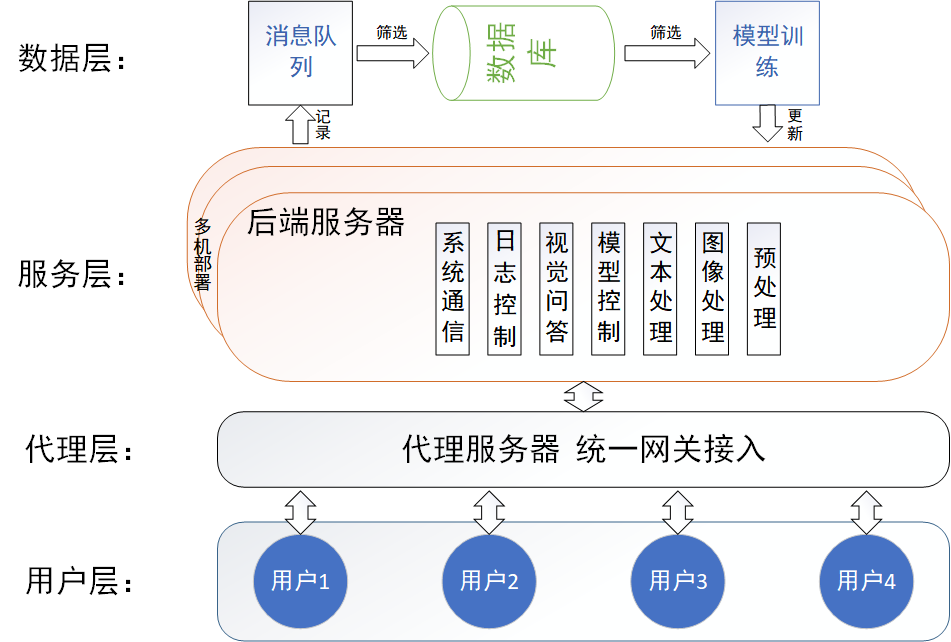
\includegraphics[width=0.8\textwidth]{Fig/myfig/chapter5/sys_framwork.png}  %scale = 0.3
	% 添加标签one_DFUAV以及图标题“XXX”,引用某图时使用\ref{xxx},其中xxx就是标签,图编号是自动生成的。
	\caption{\label{sys_framwork}总体框架} 
\end{figure}

\begin{enumerate}[topsep = 0 pt, itemsep= 0 pt, parsep=0pt, partopsep=0pt, leftmargin=0pt, itemindent=44pt, labelsep=6pt,  listparindent=22pt, label=(\arabic*)]
	\item 客户端
	
	基于Web网页端实现,用户可以通过访问网页(前端界面)上传图片信息和问题信息来和视觉问答系统进行交互。网页接收信息流后向后端服务API发起访问,并接收
	返回的回答内容并转换成文本或者语音的形式呈现给用户。
	\item 代理服务器

	面对公网开放服务时,代理服务器是客户端到后端服务器的连接桥梁,代理服务器具有路由映射组件。通过路由映射表将来自于公网的服务请求路由到后端服务器,
	访问服务器上的对应接口,并在获得服务API的接口返回数据后再发送回请求方。使用代理服务器有许多优势,首先是避免了服务器主机直接开放到公网上,防止服务被劫持。
	其次,代理服务器的负载均衡组件可以有效管理访问流量。它可以根据预设的策略将客户端的请求流量分发到后端服务器,从而避免了因流量过大而导致服务器宕机的情况。这种管理访问流量的方法可以提高系统的可用性和稳定性。
	同时,代理服务器具备的心跳检测组件可以发现故障的后端服务器,如果内网中仍有其他服务器可以正常提供服务,代理服务器可以将后续的请求路由到正常运行的服务器上,提高了服务的稳定性。
	\item 后端服务器
	
	为了提高后端服务的效率和稳定性,通常会采用单机或者多机部署的方式。后端服务主要包括系统管理模块、信息处理模块和视觉问答模块。
	其中,系统管理模块提供用户注册登录等接口,信息处理模块则提供视觉问答数据需要的转化接口,而视觉问答模块则是整个系统的核心组件,包含了各种视觉问答模型,负责接收数据并进行相应的预测和回答。
	为了更好地满足用户需求,还可以在视觉问答模块中采用缓存数据的方式,减少数据读取和存储的时间,并利用消息队列技术进行削峰、解耦以及异步处理,提高系统的响应速度和性能。
	此外,为了有效管理访问流量,代理服务器中可以添加负载均衡组件,将客户端的请求流量按策略请求分发到后端服务器,避免服务器因流量过大而出现宕机等问题,保证系统的稳定性和可用性。
\end{enumerate}

\subsection{工作数据流}
如图\ref{data_string}所示,为了更好地理解整个架构和数据流转方式,设计的模态自适应医学视觉问答系统的数据工作流主要包含了用户请求、问答信息、问答记录三个部分。要实现分别记录不同用户的问答信息并保存在文件中作为数据反馈,需要一个高效的
数据工作流处理方式。
\begin{figure}[htbp]
	% 图片居中(列居中对齐)
	\centering	
	% 包含当前路径下的Fig文件夹的图片文件
	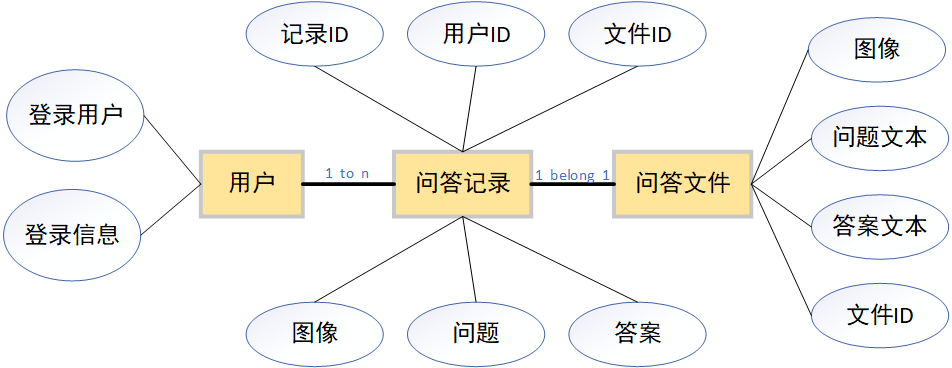
\includegraphics[width=0.8\textwidth]{Fig/myfig/chapter5/data_string.png}  %scale = 0.3
	% 添加标签one_DFUAV以及图标题“XXX”,引用某图时使用\ref{xxx},其中xxx就是标签,图编号是自动生成的。
	\caption{\label{data_string}工作数据流图示} 
\end{figure}
用户数据是系统接口收集到的用户信息和登录信息,问答记录数据记录了和用户的交互以及反馈信息,包含三种ID数据和三类问答数据,一个用户包含了许多的问答记录,所以是1 to n的关系。问答文件是问答记录的实际载体,一个问答文件对应一次问答记录,以便于在系统中进行数据整理。
\subsection{后端API服务接口设计}
设计一个合理的API接口往往包含了开发语言和框架的选择、输入输出参数和格式的确定、编写接口功能、部署服务、测试、文档化、发布等过程。

服务器端主要通过HTTP/HTTPS协议为客户端提供视觉问答接口。其中信息处理模块集成在了接口上,接口的通信格式为json,通信内容如表\ref{tab:sys_api}。
\begin{table}
    \caption{\label{tab:sys_api}后端API接口通信格式}
    \centering
    \begin{tabular}{lll}
        \hline 字段名 & 类型 & 描述  \\
        \hline code & int & 状态码  \\
		message & String & 消息 \\
		data & json & 数据 \\
        \hline
        \end{tabular}
\end{table}	
视觉问答接口是实现系统问答和提供服务的核心,在内部调用了各个算法服务,包括视觉问答算法服务,模型请求和信息处理中的各种算法。客户端通过HTTP经代理发送请求给后端服务器,
并携带想要提问的图像和文本问题,后端服务器将最终的回答返回给客户端。

\section{系统综合设计与实现}
\subsection{系统架构}
如表\ref{tab:sys_lib},要搭建实现一个在线医学视觉问答系统,并保证其服务的稳定性、可靠性、闭环性以及安全性,需要一个较好的集成化设计,框架分用户层、代理层、服务层、数据层进行了设计。

\begin{table}
    \caption{\label{tab:sys_lib}主要使用的服务框架}
    \centering
    \begin{tabular}{llll}
        \hline 用户层 & 代理层 & 服务层 & 数据层 \\
        \hline Gradio & Coplar & Docker & Flask \\
        \hline
        \end{tabular}
\end{table}	
\begin{enumerate}[topsep = 0 pt, itemsep= 0 pt, parsep=0pt, partopsep=0pt, leftmargin=0pt, itemindent=44pt, labelsep=6pt, listparindent=22pt, label=(\arabic*)]
	\item Gradio
	
	Gradio是一个基于Web的交互式界面构建框架,可以用于构建机器学习模型的演示和应用。使用Gradio可以将模型部署为具有自定义用户界面的Web应用程序。
	\item Coplar
	
	Coplar框架是一个用于提供内网穿透服务的应用框架,用于解决在内网环境下的外部访问问题,例如在企业内部网络中,往往存在一些需要从外网访问的资源,例如Web服务、数据库等,但这些资源由于被部署在内网中,因此无法直接通过公网IP进行访问。
	Coplar内网穿透服务可以将内网资源映射到公网上,从而实现对内网资源的远程访问。
	\item Docker
	
	Docker是一种容器化平台和服务,可以帮助开发人员和系统管理员在虚拟化环境中轻松地构建、部署和运行应用程序。Docker容器还提供了一个隔离环境,使得应用程序可以在一个独立的运行环境中运行,不受其他应用程序或系统资源的影响。
	\item Flask
	
	Flask框架的核心是一个WSGI(Web Server Gateway Interface)应用程序,其实现非常简单,一般只有几个Python文件,其中包括了应用程序、路由、视图函数、模板、静态文件等。Flask通过装饰器机制实现路由映射,使开发人员可以通过定义路由和视图函数的方式,轻松地实现各种HTTP请求的响应处理。
	有利于收集用户数据,建立数据库和服务之间的快速通路。
\end{enumerate}

\subsection{系统管理}
系统管理主要是在数据以及通信层管理包括控制模型调用、访问控制、日志记录等系统功能。并通过编程和逻辑设计解决一系列部署中会遇到的问题。例如如何调配资源和模型对处理访问申请,如何在用户
访问过程中进行并行的日志记录,如何监控异常行为,返回错误信息等。管理模式如图\ref{sys_control}。
\begin{figure}[htbp]
	% 图片居中(列居中对齐)
	\centering	
	% 包含当前路径下的Fig文件夹的图片文件
	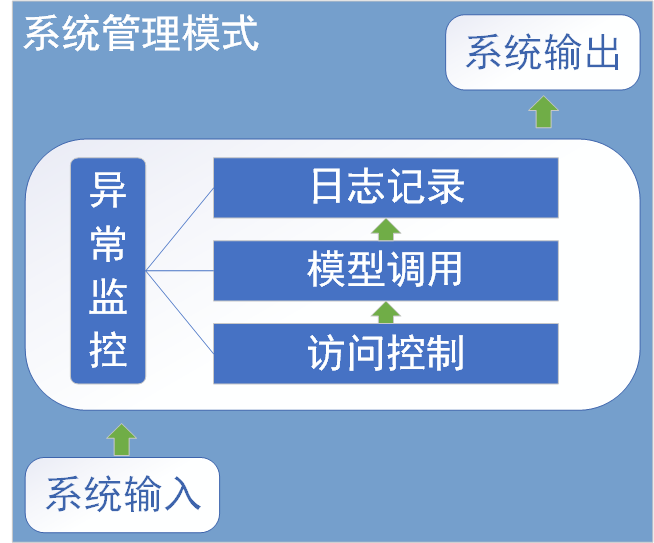
\includegraphics[width=0.5\textwidth]{Fig/myfig/chapter5/sys_control.png}  %scale = 0.3
	% 添加标签one_DFUAV以及图标题“XXX”,引用某图时使用\ref{xxx},其中xxx就是标签,图编号是自动生成的。
	\caption{\label{sys_control}系统管理模式} 
\end{figure}

\subsection{信息处理}
信息处理单元一般都集成在接口处,处理包括读取用户请求输入的图像数据和文本数据。由于在线系统的图片输入一般会分成互联网统一资源定位符(url)或者本地上传形式,所以都需要先将其统一读取成二进制形式交由模型处理。
文本作为一个字符串,直接由模型读取并转化成响应的token。以下是系统中会遇到的信息以及其格式和处理方法。
\begin{table}
    \caption{\label{tab:linkvqa}接口信息处理}
    \centering
    \begin{tabular}{l|l}
        \hline 信息内容 & 接口信息处理操作 \\
        \hline \multirow{3}*{图像操作} & 按84×84进行裁剪(AE) \\
		& 按128×128进行裁剪(MAML) \\
		& 按250×250进行裁剪 (CLIP) \\
		\hline \multirow{2}*{文本操作} & 语种识别(langdetect) \\
		& 语言翻译(API) \\
        \hline
        \end{tabular}
\end{table}	

\subsection{视觉问答}
视觉问答又是模型服务端,也就是模型的预测函数。通常由模型结构+加预训练好的参数构成,在调用问答服务时,模型会处理接口端传输来的图像和文本信息,然后预测输出并返回;通常为了保证深度学习模型和其环境的稳定性,
主流上都会使用Docker组件对模型以及所需要的环境进行封装并打包到第一个可移植的容器中。以便在任何地方都可以轻松部署。Docker容器是镜像运行的实例。
负责管理容器的创建、启动、停止等操作。视觉问答接口请求如表\ref{tab:linkvqa}:
\begin{table}
    \caption{\label{tab:linkvqa}视觉问答接口}
    \centering
    \begin{tabular}{l|l}
        \hline 接口名 & 视觉问答 \\
        \hline 请求协议 & HTTP\textbackslash HTTPS \\
		请求方法 & Post \\
		请求url & \textbackslash post \\
		携带参数 & 图像数据、文本数据 \\
		返回结果 & 文字和不确定估计结果 \\
        \hline
        \end{tabular}
\end{table}	

为了简化系统管线设计,如表\ref{tab:linkfeedback}数据反馈接口采用视觉问答接口同样的服务方式:
\begin{table}
    \caption{\label{tab:linkfeedback}数据反馈接口}
    \centering
    \begin{tabular}{l|l}
        \hline 接口名 & 数据反馈 \\
        \hline 请求协议 & HTTP\textbackslash HTTPS \\
		请求方法 & Feedback \\
		请求url & \textbackslash Feedback \\
		携带参数 & 图像数据、文本数据、反馈标记 \\
		返回结果 & 感谢性图文描述 \\
        \hline
        \end{tabular}
\end{table}	

\subsection{前端界面}
在前端的编写使用中最注重的就是可视化。Gradio是一个轻量级的工具,主要用于快速编写可视化的Demo,搭建模型的Demo并部署深度学习模型。但其本身并不具备模型管理功能,必须采用其他的方式管理模型。
因而后端为了与前端有更好的区分,采用了Flask框架编写。

如图\ref{demo_sum},前端用户交互界面的设计采用了VQA—Demo最常用的双流输入-输出的方式,也就是一侧负责模型输入,一侧负责模型输出。这种设计更具有和模型对话的效果,可以提高用户的交互体验。此外,为了更好地收集用户反馈,在输入栏下方设计了反馈栏,这样便于用户同时将反馈信息输入给模型。。
\begin{figure}[htbp]
	% 图片居中(列居中对齐)
	\centering	
	% 包含当前路径下的Fig文件夹的图片文件
	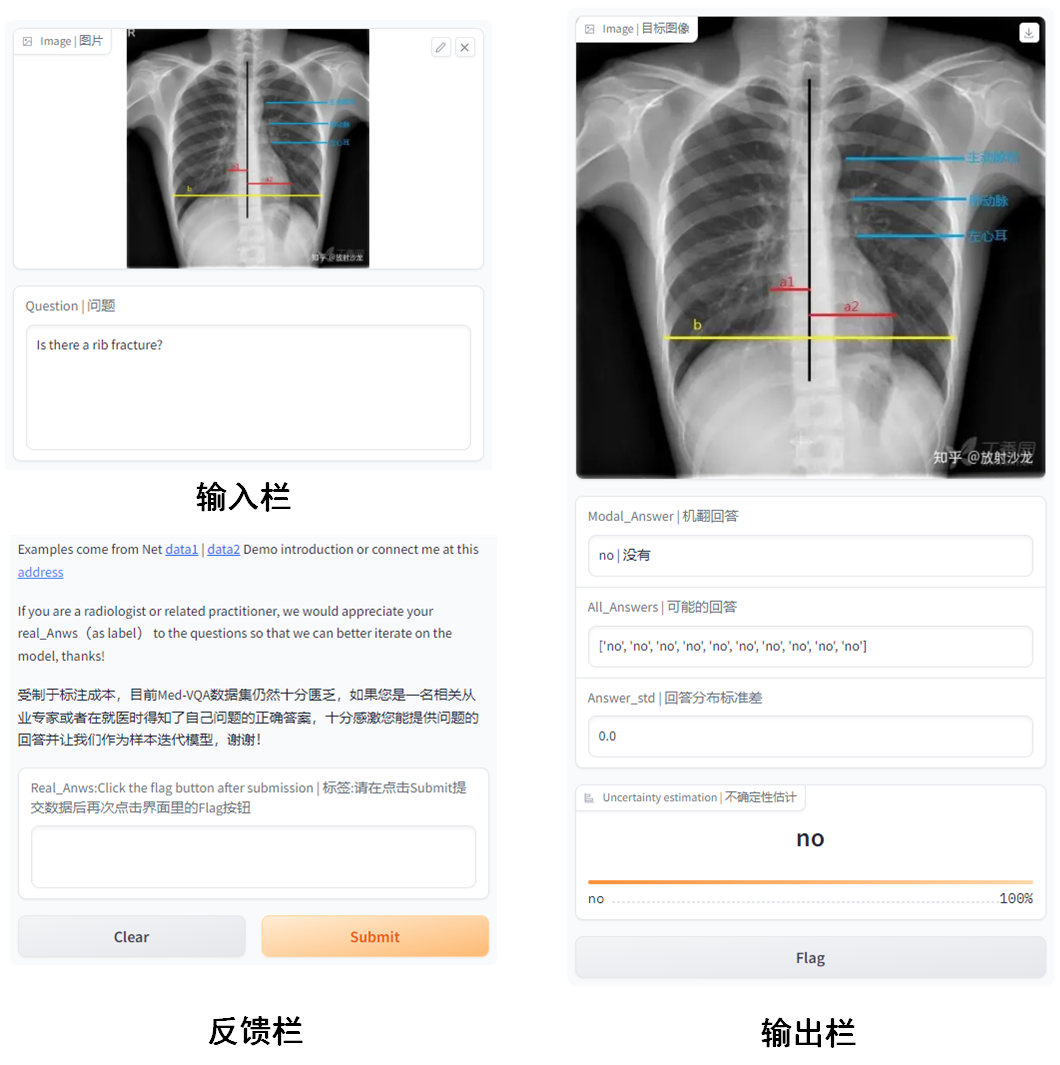
\includegraphics[width=0.8\textwidth]{Fig/myfig/chapter5/demo_sum.png}  %scale = 0.3
	% 添加标签one_DFUAV以及图标题“XXX”,引用某图时使用\ref{xxx},其中xxx就是标签,图编号是自动生成的。
	\caption{\label{demo_sum}用户交互界面} 
\end{figure}

如图\ref{demo_example}为了更方便用户快速上手该系统,Demo还在最后设置了三类输入样例、8组对话样例的样例栏。方便用户在进入界面后可以快速使用这些例子进行体验。
\begin{figure}[htbp]
	% 图片居中(列居中对齐)
	\centering	
	% 包含当前路径下的Fig文件夹的图片文件
	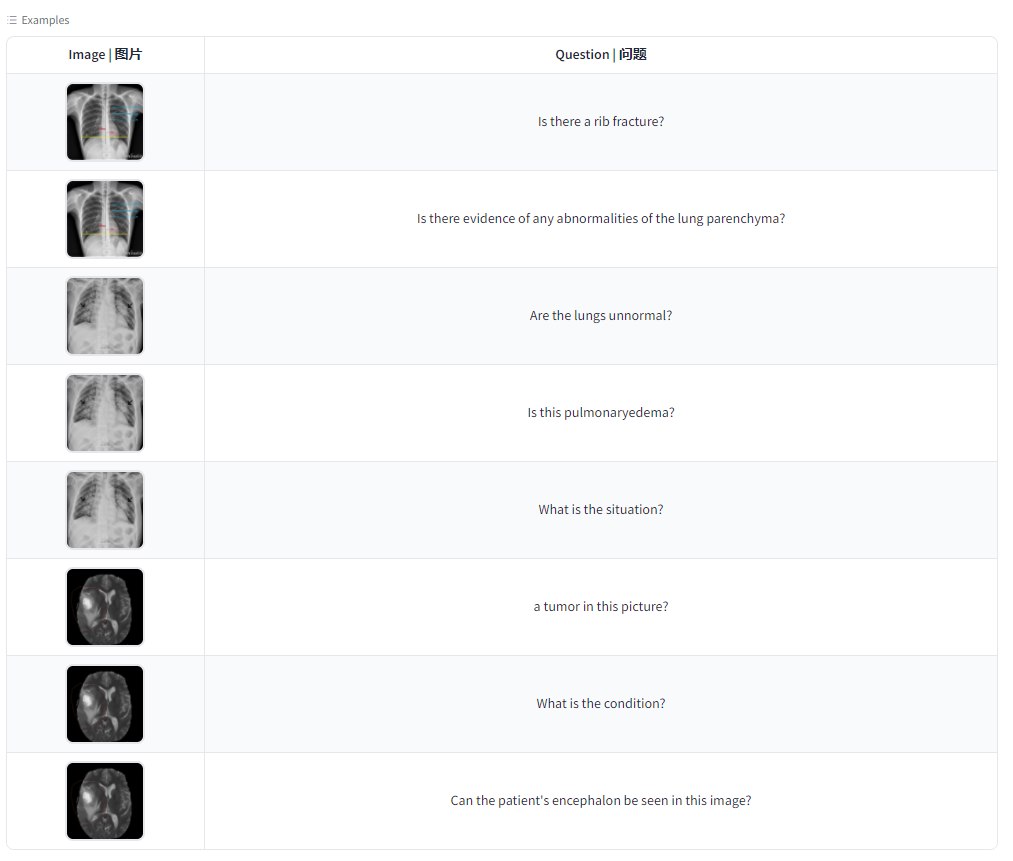
\includegraphics[width=0.8\textwidth]{Fig/myfig/chapter5/demo_example.png}  %scale = 0.3
	% 添加标签one_DFUAV以及图标题“XXX”,引用某图时使用\ref{xxx},其中xxx就是标签,图编号是自动生成的。
	\caption{\label{demo_example}交互样例栏} 
\end{figure}
% \begin{figure}[htbp]
% 	\begin{minipage}{0.5\linewidth}
% 		\centering	
% 		% 包含当前路径下的Fig文件夹的图片文件
% 		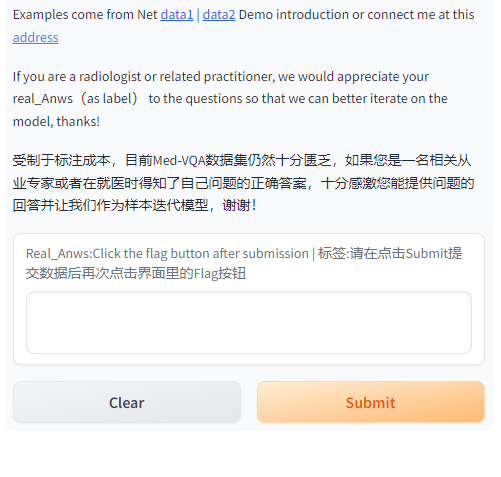
\includegraphics[width=0.8\textwidth]{Fig/myfig/chapter5/demo_feedback.png}  %scale = 0.3
% 		% 添加标签one_DFUAV以及图标题“XXX”,引用某图时使用\ref{xxx},其中xxx就是标签,图编号是自动生成的。
% 		\caption{\label{demo_feedback}Demo反馈栏} 	
% 	\end{minipage}
% 	% 图片居中(列居中对齐)
% 	\begin{minipage}{0.5\linewidth}
% 		\centering	
% 		% 包含当前路径下的Fig文件夹的图片文件
% 		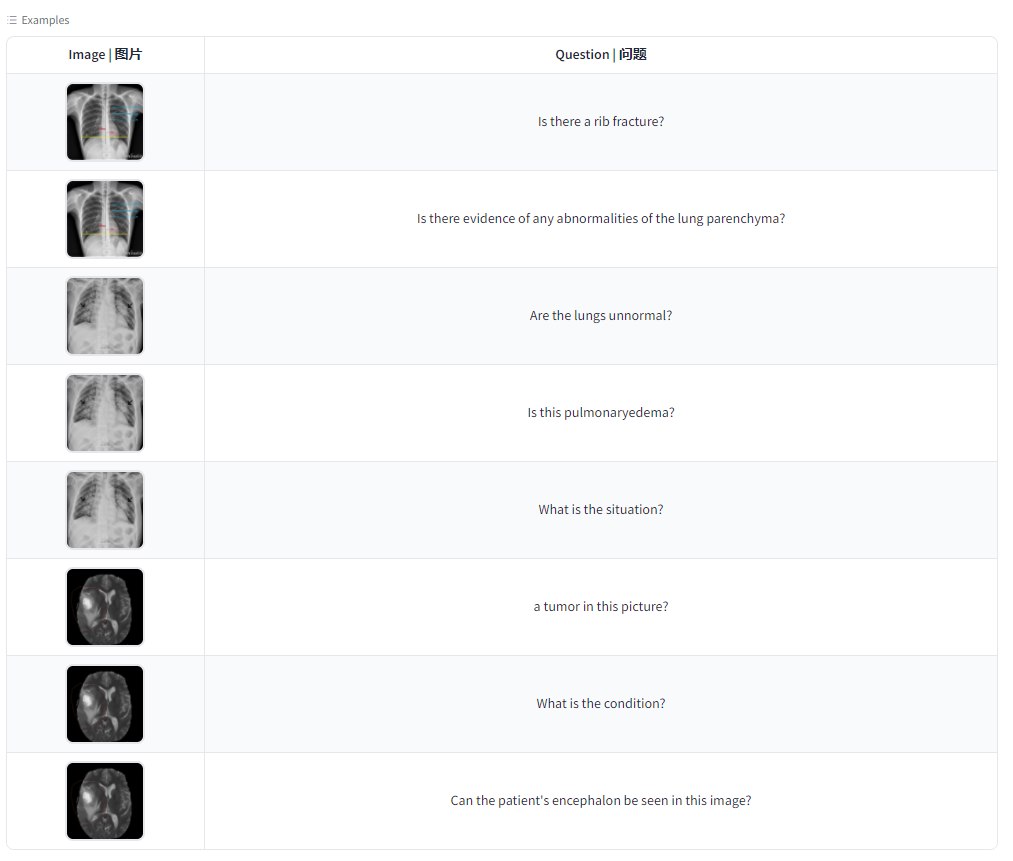
\includegraphics[width=0.8\textwidth]{Fig/myfig/chapter5/demo_example.png}  %scale = 0.3
% 		% 添加标签one_DFUAV以及图标题“XXX”,引用某图时使用\ref{xxx},其中xxx就是标签,图编号是自动生成的。
% 		\caption{\label{demo_example}Demo样例栏} 
% 	\end{minipage}
% \end{figure}

\section{系统测试}
\subsection{系统接口测试}
本小节介绍了如何使用常见的接口测试工具Postman来测试问答接口。在测试时,需要使用HTTP协议,请求方式为POST,同时请求需要携带图像信息和问题文本这两个参数。
测试的URL路径为/post。请求格式JSON例子如图\ref{post}。
\begin{figure}[htbp]
	% 图片居中(列居中对齐)
	\centering	
	% 包含当前路径下的Fig文件夹的图片文件
	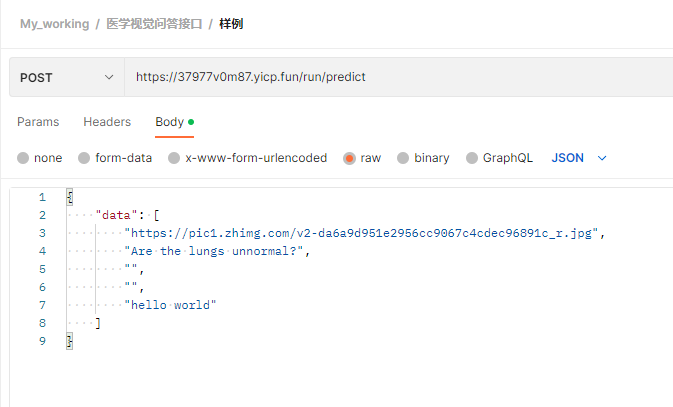
\includegraphics[width=0.8\textwidth]{Fig/myfig/chapter5/post.png}  %scale = 0.3
	% 添加标签one_DFUAV以及图标题“XXX”,引用某图时使用\ref{xxx},其中xxx就是标签,图编号是自动生成的。
	\caption{\label{post}向API发送请求} 
\end{figure}

测试的返回结果为文本。经过测试返回结果如图\ref{get},本次测试获得了接口返回的json数据,其中包含了模型回答、
模型不确定性预测、结果方差以及不确定标签评估等信息,与预期结果一致。
\begin{figure}[htbp]
	% 图片居中(列居中对齐)
	\centering	
	% 包含当前路径下的Fig文件夹的图片文件
	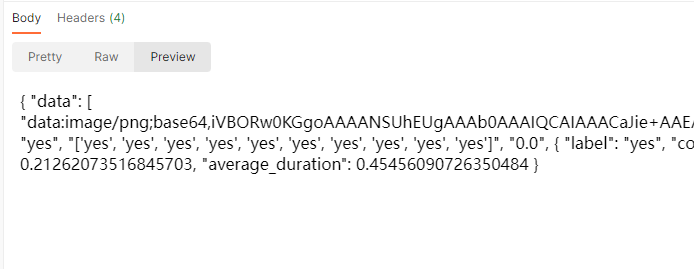
\includegraphics[width=0.8\textwidth]{Fig/myfig/chapter5/post_get.png}  %scale = 0.3
	% 添加标签one_DFUAV以及图标题“XXX”,引用某图时使用\ref{xxx},其中xxx就是标签,图编号是自动生成的。
	\caption{\label{get}获得API返回数据} 
\end{figure}

\subsection{系统响应测试}
以使用单MEMSA模型进行检索式回答为例,系统响应时间即为处理用户请求的时间,包括网络延迟、接口响应时间、模型预测以及返回时间等等,反应了一个系统的快速性,同时也是良好人机交互体验的基础。
如表\ref{tab:timerep}是用户对每个模型进行3次请求的响应时间统计,可见本系统在使用不同模型时都有较为稳定的响应速度,大约只需要四分之一秒即可完成请求的处理并返回,属于具备毫秒级的响应能力的系统。
由于不同用户间的网络时延无法稳定估计,故在此处不予以测量。
\begin{table}
	\caption{\label{tab:timerep}系统响应时长 | 单位:秒}
	\centering
	\small
	\begin{tabular}{c|c|c|c|c|c}
		\hline 搭载模型 & 测试序数 & 接口响应时长 & 模型响应时长 & 总响应时长 & 平均响应时长 \\
		\hline \multirow{3}{*}{$\begin{array}{l}\text { MEMSA-MLP } \\
		\text { (Med-RAD) }\end{array}$} & 1 & 0.01 & 0.24 & 0.25 & \multirow{3}{*}{0.27} \\
		& 2 & 0.003 & 0.25 & 0.25 & \\
		& 3 & 0.005 & 0.29 & 0.30 & \\
		\hline \multirow{3}{*}{$\begin{array}{l}\text { MEMSA-BMLP } \\
		\text { (Med-RAD) }\end{array}$} & 1 & 0.01 & 0.27 & 0.28 & \multirow{3}{*}{0.27} \\
		& 2 & 0.005 & 0.26 & 0.27 & \\
		& 3 & 0.003 & 0.27 & 0.27 & \\
		\hline \multirow{3}{*}{$\begin{array}{l}\text { MEMSA-MLP } \\
		\text { (SLAKE) }\end{array}$} & 1 & 0.006 & 0.25 & 0.26 & \multirow{3}{*}{0.25} \\
		& 2 & 0.004 & 0.24 & 0.24 & \\
		& 3 & 0.006 & 0.25 & 0.26 & \\
		\hline \multirow{3}{*}{$\begin{array}{l}\text { MEMSA-BMLP } \\
		\text { (SLAKE) }\end{array}$} & 1 & 0.009 & 0.27 & 0.28 & \multirow{3}{*}{0.27} \\
		& 2 & 0.003 & 0.26 & 0.26 & \\
		& 3 & 0.005 & 0.26 & 0.27 & \\
		\hline
	\end{tabular}
\end{table}	


% \begin{enumerate}[topsep = 0 pt, itemsep= 0 pt, parsep=0pt, partopsep=0pt, leftmargin=0pt, itemindent=44pt, labelsep=6pt, listparindent=22pt, label=(\arabic*)]
% 	\item 可用性/稳定性
	
% 	主要由系统是否能够24小时稳定运行,系统是否能够承受高并发访问,系统是否能够快速响应用户请求这三样指标。
% 	\item 响应时间
	
% 	系统响应时间即为处理用户请求的时间,包括网络延迟、接口响应时间、模型预测以及返回时间等等,如表\ref{tab:timerep}是用户对每个模型进行3次请求的响应时间统计:
% 	\begin{table}
% 		\caption{\label{tab:timerep}系统响应时长}
% 		\centering
% 		\small
% 		\begin{tabular}{c|c|c|c|c|c}
% 			\hline 模型 & 测试序数 & 接口响应时长 & 模型响应时长 & 总响应时长 & 平均响应时长 \\
% 			\hline \multirow{3}{*}{$\begin{array}{l}\text { MEMSA-MLP } \\
% 			\text { (Med-RAD) }\end{array}$} & 1 & 0.01 & 0.24 & 0.25 & \multirow{3}{*}{0.27} \\
% 			& 2 & 0.003 & 0.25 & 0.25 & \\
% 			& 3 & 0.005 & 0.29 & 0.30 & \\
% 			\hline \multirow{3}{*}{$\begin{array}{l}\text { MEMSA-BMLP } \\
% 			\text { (Med-RAD) }\end{array}$} & 1 & 0.01 & 0.27 & 0.28 & \multirow{3}{*}{0.27} \\
% 			& 2 & 0.005 & 0.26 & 0.27 & \\
% 			& 3 & 0.003 & 0.27 & 0.27 & \\
% 			\hline \multirow{3}{*}{$\begin{array}{l}\text { MEMSA-MLP } \\
% 			\text { (SLAKE) }\end{array}$} & 1 & 0.006 & 0.25 & 0.26 & \multirow{3}{*}{0.25} \\
% 			& 2 & 0.004 & 0.24 & 0.24 & \\
% 			& 3 & 0.006 & 0.25 & 0.26 & \\
% 			\hline \multirow{3}{*}{$\begin{array}{l}\text { MEMSA-BMLP } \\
% 			\text { (SLAKE) }\end{array}$} & 1 & 0.009 & 0.27 & 0.28 & \multirow{3}{*}{0.27} \\
% 			& 2 & 0.003 & 0.26 & 0.26 & \\
% 			& 3 & 0.005 & 0.26 & 0.27 & \\
% 			\hline
% 		\end{tabular}
% 	\end{table}	
% 	\item 可扩展性
	
% 	如图
% 	\item 安全性和可靠性
	
% 	该系统所处的服务器与用户之间的通信经过Https加密传输,HTTPS (Hyper Text Transfer Protocol Secure)是一种基于加密传输的HTTP协议。
% 	它使用SSL(Secure Socket Layer)或TLS(Transport Layer Security)协议进行加密,保证通信过程中数据的安全性和完整性。使用HTTPS可以有效地保护通信过程中的数据安全和隐私,防止信息被窃听和篡改。
% 	这极大保证了系统在通信时的信息安全,同时完整的信息传递也使得模型能够准确接收用户请求,提高了系统的可靠性。
% \end{enumerate}

\section{本章小结}
本章首先介绍了模态自适应系统的技术路线和设计原理,分析了系统如何针对输入适应性采取检索或生成式问答策略,并对两类模型模型的问答进行了比较。
接着针对目前Med-VQA通用场景在评估了各个经典机器学习算法的性能,并选用最优的算法作为控制交互模型的自适应方法,紧接着又介绍了云端在线系统的设计过程,从分析用户功能需求的角度确定系统需要实现的服务目标并以此设计出
在线系统框架,从而设计数据工作流和相应后端服务支持。然后分别从系统架构、系统管理、信息处理、视觉问答以及前端页面五个部分介绍了从
设计到实现的过程。最后,通过网络测试工具对模型服务进行了在线测试,得到了正确的返回,同时测试系统各模型的响应时间。
验证了这个在线系统的快速性和可靠性,为整个系统的实用化打下基础。

综上,本章通过分别设计和实现了模态自适应系统和在线系统设计部署,让一个本地模型可以通过互联网远程地为用户们提供医疗视觉问答服务,并适应
用户的实时反馈和交互,是一个可以实现在线学习和更新的系统,具备一定的实际意义和创新价值。













